%%%%%%%%%%%%%%%%%%%%%%%%%%%%%%%%%%%%%%%%%%%%%%%%%%%%%%%%%%%%%%%%%%
% Rascunho Quatro do artigo para o EduComp 2025
%%%%%%%%%%%%%%%%%%%%%%%%%%%%%%%%%%%%%%%%%%%%%%%%%%%%%%%%%%%%%%%%%%%%

\documentclass[12pt]{article}
\usepackage{sbc-template}
\usepackage{graphicx,url}
\usepackage[brazil]{babel}   
\usepackage[utf8]{inputenc} 
\usepackage{verbatim}

% pacote para citações entre aspas
\usepackage{dirtytalk}
     
% Tabela com linhas de espessuras diferentes
\usepackage{booktabs}

% Colunas de largura fixa, com diversos alinhamentos do texto (centralizado, direita, esquerda)
% Exemplo de uso: C{2.5cm}
\usepackage{array}
\newcolumntype{C}[1]{>{\centering\arraybackslash}m{#1}}
\newcolumntype{R}[1]{>{\raggedleft\arraybackslash}m{#1}}
\newcolumntype{L}[1]{>{\raggedright\arraybackslash}m{#1}}


\sloppy

\title{Aplicação da Teoria de Resposta ao Item (TRI) na classificação de questões de programação em um juiz online}

\author{Oculto para revisão}

\address{Oculto para revisão
  \email{Oculto para revisão}
}

\begin{document}

\maketitle

\begin{resumo}
A Teoria de Resposta ao Item (TRI) permite modelar a probabilidade de um indivíduo responder corretamente a uma questão, considerando tanto sua habilidade quanto a dificuldade do item. No caso de questões de programação em juízes online, elas produzem dois tipos de feedback: certo ou errado. Assim, elas podem ser modeladas como itens dicotômicos, seguindo os princípios da TRI. Este estudo aplica algoritmos de aprendizado de máquina para classificar parâmetros da TRI, com o objetivo de prever a taxa de erro e a capacidade de discriminação de questões de escrita de código no contexto de uma disciplina introdutória de programação. Nos experimentos, os classificadores apresentaram pior desempenho ao discriminar entre três categorias, em comparação com duas. Neste último caso, foi alcançado um f1-score de 0,81 para prever a taxa de erro e 0,89 para a capacidade de discriminação.
\end{resumo}

\begin{abstract}
The Item Response Theory (IRT) allows for modeling the probability of an individual correctly answering a question, considering both their ability and the item's difficulty. In the case of programming questions in online judges, they produce two types of feedback: correct or incorrect. Thus, they can be modeled as dichotomous items, following the principles of IRT. This study applies machine learning algorithms to classify IRT parameters, aiming to predict the error rate and the discrimination ability of coding questions in the context of an introductory programming course. In the experiments, the classifiers performed worse when distinguishing between three categories, compared to two. In the latter case, an f1-score of 0,61 was achieved for predicting the error rate and 0,88 for the discrimination ability.
\end{abstract}

%========================================================================================

\section{Introdução}

A Teoria de Resposta ao Item (TRI) tem se consolidado como uma abordagem estatística no campo da avaliação educacional e psicológica, possibilitando compreender e melhorar a precisão na medição de habilidades ou traços latentes --- características individuais que não podem ser diretamente observadas, como habilidade matemática, compreensão de leitura, ou proficiência em programação \cite{Liz2020,pasquali2003}. A precisão na estimativa dessas habilidades depende não apenas do modelo teórico empregado, mas também da qualidade dos itens avaliativos utilizados.

No contexto do ensino-aprendizagem de programação, um juiz online (JO) é um sistema projetado para avaliação automática do código-fonte enviado pelos alunos como resposta a exercícios cadastrados \cite{Wasik2018}. Para a correção automática, um JO usa tipicamente casos de teste, que são um conjunto de entradas e as respectivas saídas esperadas. O código submetido por um aluno é considerado como correto se, para cada entrada testada, fornecer como saída os resultados correspondentes cadastrados pelo instrutor \cite{elrik2022}. Embora do ponto de vista do estudante as questões de programação possam seguir um modelo discursivo de resposta, do ponto de vista da correção, elas são dicotômicas, por terem apenas duas possibilidades de resposta: certo, quando passam em todos os casos de teste, ou errado, quando não passa em pelo menos um. Embora alguns JOs considerem pontuações parciais proporcionais ao número de casos de teste bem sucedidos, esse cenário não é comum e por isso não é abordado neste trabalho.

Instrutores de disciplinas de programação introdutória têm empregado diversos JOs para aplicar avaliações. Nesses casos, o professor escolhe algumas questões disponíveis no banco de dados do JO para serem resolvidas durante o tempo que, comumente, é destinado à aula \cite{jackson2023}. Normalmente, são sorteadas questões diferentes para cada aluno, para evitar plágio. No entanto, neste sorteio, o sistema pode desbalancear (para cima ou para baixo) a dificuldade da prova de um aluno, pois o professor não pode garantir a uniformidade de desafio para todos os alunos em um ambiente aleatório \cite{marcos2021}.

Com este cenário, a aplicação da TRI na classificação de questões de prova se torna uma grande oportunidade de adaptar a avaliação do ensino-aprendizagem de programação a cada pessoa, considerando a curva de evolução e as lacunas que cada estudante possa vir a ter, personalizando o ensino de programação. Como a TRI trabalha com questões de múltipla escolha, em sua maioria --- como o Exame Nacional do Ensino Médio (Enem) e o Exame Nacional de Desempenho dos Estudantes (Enade), é necessário fazer uma adaptação para contemplar o contexto de juízes online para o ensino de programação: embora os itens tratados sejam dicotômicos, como apresentado antes, a resolução por parte dos estudantes envolve um discurso --- no caso, a produção de código.

Diante do exposto, o objetivo deste presente trabalho é adaptar a Teoria de Resposta ao Item para predizer os itens classificadores de questões de programação cadastrados em um juiz online, com base em turmas de programação introdutórias em cursos que não são oriundos da Computação, utilizando técnicas aplicadas na área de aprendizado de máquina. Em uma visão macro, tal objetivo pode ser ramificado nas seguintes questões de pesquisa:

\begin{description}
    \item [QP1:] É possível determinar a discriminação de uma questão com os indicadores disponíveis? 
    \item [QP2:] A TRI consegue maximizar a precisão da taxa de erro?
    \item [QP3:] É possível afirmar que existe correlação entre dificuldade e discriminação?
\end{description}

A partir das questões de pesquisa, foram definidas as vertentes norteadoras do trabalho, divididas nestas etapas: revisão da literatura; extração de questões de uma base anônima pública e construção da base de dados; definição do cálculo da discriminação e das métricas de avaliação; e treinamento dos modelos de classificação e regressão.

%======================================================================

\section{Trabalhos Relacionados}

% Esta seção foca na revisão da literatura sobre os nortes utilizados neste trabalho - a fundamentação teórica da TRI e a apreciação de trabalhos anteriores que não utilizaram a TRI, porém focaram na classificação de dificuldade de questões de programação.

Esta seção aborda os trabalhos anteriores realizados em duas frentes de pesquisa: a fundamentação teórica da TRI e a classificação de dificuldade de questões de programação.

\subsection{Teoria de Resposta ao Item}

A TRI é um dos principais modelos estatísticos utilizados na psicometria e na educação para avaliar habilidades latentes, ou seja, características individuais que não podem ser diretamente observadas, como habilidade matemática, compreensão de leitura, ou proficiência em programação \cite{Liz2020}. A TRI foi desenvolvida para superar limitações da Teoria Clássica dos Testes (TCT), que depende fortemente da amostra utilizada para estimar a dificuldade e discriminação dos itens e foca nos escores totais dos testes, em vez de analisar cada item individualmente \cite{Valle2000}.

A TRI se baseia na ideia de que a probabilidade de um aluno responder corretamente a um item (questão) depende de um conjunto de parâmetros do item e do nível de habilidade do aluno. Os modelos da TRI incluem de um a quatro parâmetros: taxa de erro, discriminação, acerto e erro ao acaso \cite{Klein2009}. Como as respostas de questões de programação demandam escrita de código, e não escolha de uma opção entre alternativas, os dois últimos parâmetros têm baixo impacto na dificuldade do item, por isso não foram usados neste trabalho. Os dois parâmetros utilizados foram estes \cite{Liz2020}:

\begin{itemize}
    \item Taxa de Erro ($b$): nível de habilidade necessária para que a chance de responder corretamente a uma questão seja de 50\%. Itens com alto valor de taxa de erro exigem maior proficiência para serem respondidos corretamente.
    
    \item Discriminação ($a$): mede a capacidade do item de distinguir entre indivíduos com diferentes níveis de habilidade. Itens com alta discriminação diferenciam bem entre alunos mais e menos proficientes.
\end{itemize}

A taxa de erro também é designada na literatura pelo termo \say{dificuldade}. Porém, neste trabalho, preferimos reservar esse termo para nos referir aos níveis quantificáveis do sucesso de uma pessoa em lidar com uma determinada demanda. No contexto de programação, a dificuldade pode ser expressa por diferentes métricas de esforço na interação dos alunos com as questões cadastradas em um JO, tais como taxa de respostas incorretas, tempo mediano de resposta, número de tentativas \cite{elrik2022}, entre outras, como será discutido na Seção~\ref{sec:revlit:dificuldade}.

A TRI permite que os parâmetros dos itens sejam independentes das amostras utilizadas, ou seja, as estimativas de taxa de erro e discriminação dos itens são mais estáveis e podem ser aplicadas a diferentes grupos de estudantes \cite{Valle2000}. Ademais, a TRI possibilita a aplicação de Testes Adaptativos Informatizados, nos quais itens são ajustados em tempo real ao nível de habilidade do aluno, proporcionando uma avaliação personalizada \cite{Liz2020}. Esses benefícios, embora não abordados neste trabalho, motivam a aplicação da TRI em ambientes educacionais como JOs, nos quais é essencial ajustar a dificuldade das questões conforme a evolução das habilidades do aluno.

\subsection{Classificação de dificuldade de questões de programação sem TRI} \label{sec:revlit:dificuldade}

Trabalhos anteriores já abordaram o tema da predição da dificuldade de questões de programação sob várias perspectivas. \cite{pelanek2022complexity} abordaram a diferenciação entre complexidade e dificuldade de itens em sistemas de aprendizado. %, com ênfase nas aplicações práticas desses conceitos em sequenciamento de itens, modelagem de estudantes e gerenciamento de conteúdo. 
Eles destacam que, embora esses conceitos sejam frequentemente usados de forma intercambiável, há uma distinção fundamental entre eles. A complexidade é vista como uma propriedade intrínseca de uma tarefa, determinada por sua estrutura interna, enquanto a dificuldade está relacionada à interação entre o aluno e a tarefa, medindo o desempenho dos alunos.

Em outro ramo, \cite{santos2019} abordaram a classificação da dificuldade de questões de programação com base na inteligibilidade de seus enunciados. Utilizando algoritmos de aprendizado de máquina, o estudo investiga como características linguísticas e semânticas dos enunciados podem influenciar a percepção de dificuldade pelos estudantes. Os resultados indicaram que a inteligibilidade do enunciado é um fator relevante para predizer a dificuldade de questões, especialmente em uma disciplina de programação para iniciantes, em que a clareza do texto afeta significativamente o desempenho dos alunos.

Em seguida, \cite{marcos2021} investigaram como atributos do código de solução podem ser usados para classificar a dificuldade de questões de programação em juízes online. Com base em métricas de complexidade e desempenho dos alunos, eles aplicaram algoritmos de aprendizado de máquina para prever níveis de dificuldade das questões. Ao final, o estudo revelou que métricas como número de linhas de código, complexidade ciclomática e uso de estruturas específicas são úteis para identificar questões fáceis ou difíceis, indicando viabilidade de prever automaticamente a dificuldade, ajudando educadores a ajustar o nível de desafios propostos.

Posteriormente, \cite{elrik2022} avaliaram métodos automáticos para prever a dificuldade de questões de programação, utilizando métricas extraídas diretamente do código de solução, além de utilizar outras métricas para expressar a dificuldade, como tempo de codificação, número de testes e número de submissões. Notou-se que 96\% das correlações entre métricas individuais e dificuldade foram fracas ou inexistentes; apenas 4\% apresentaram correlação moderada, e nenhuma foi considerada forte.

Por fim, \cite{jackson2023} exploraram a relação entre a complexidade de questões de programação em juízes online e a dificuldade enfrentada pelos alunos ao resolvê-las, utilizando-se da correlação entre métricas de complexidade do código (linhas de código, número de variáveis, etc.) e métricas de dificuldade (tempo de resolução, número de tentativas) aliada aos modelos de aprendizado de máquina (classificação e regressão) para prever as métricas de dificuldade com base nas de complexidade.

Contudo, os trabalhos anteriores usaram a TCT como base da predição. Por sua vez, este trabalho adota uma abordagem da TRI. Ela possui alguns pontos mais avançados do que a TCT, como o cálculo dos parâmetros de avaliação, que independe da amostra de sujeitos utilizada; e também permite fazer uma relação entre itens de teste e níveis de traços individuais, o que auxilia no uso de melhores itens para se realizar a avaliação. Além disso, a análise conduzida englobou um período de observação maior, com mais dados disponíveis para serem analisados.

%===========================================================
\section{Metodologia}

Nesta seção, são descritas a base de dados de questões usada como amostra, as variáveis utilizadas e a forma de treinamento dos algoritmos de aprendizado de máquina aplicados.

% marcos e jackson
\subsection{Base de questões de programação}

Neste estudo, foi utilizada uma base pública anonimizada contendo dados de interação de estudantes fora da área de Computação com um JO aplicado em uma disciplina introdutória de programação em uma universidade pública brasileira. As questões foram aplicadas em exames presenciais realizados entre os períodos letivos de 2016 ao primeiro semestre de 2024, com exclusão do ano de 2020, quando foram aplicados remotamente em função da pandemia de Covid-19. Em seguida, foram excluídas questões que tinham menos de 16  respostas, conforme \cite{marcos2021}. No final desses filtros, a amostra deste estudo foi composta por 711 questões resolvidas por estudantes em laboratório de informática, sob a supervisão de algum instrutor.

\subsection{Variáveis independentes e dependentes}

Neste trabalho, as variáveis independentes exprimem a complexidade de uma questão, conforme detalhado em \cite{elrik2022}. Elas independem da interação do aluno com as questões e consistem em atributos extraídos a partir do código de solução fornecido pelo instrutor no JO, tais como número de operadores e número de linhas lógicas. Ao todo, foram extraídos 63 atributos da base de questões usando scripts baseados no trabalho de \cite{marcos2021}.\footnote{\url{https://anonymous.4open.science/r/questions-irt-calculator-D6DE/README.md}}

\subsection{Variáveis dependentes}

Neste estudo, foram empregadas como variáveis dependentes as métricas de dificuldade de uma questão, obtidas através da interação dos estudantes com as questões, registradas nos arquivos de logs do JO. Ao todo, foram definidas 13 variáveis dependentes. Dez delas foram tomadas a partir de \cite{jackson2023}, enquanto uma delas foi adaptada: em vez de taxa de corretude, renomeamos para taxa de erro, buscando otimizar os cálculos dos parâmetros da TRI. As outras duas foram os parâmetros da TRI: taxa de erro e discriminação. A Tabela~\ref{tab:metricas_dificuldade} descreve sucintamente cada variável.

\begin{table}[!h]
    \centering
    \scriptsize
    \caption{Variáveis dependentes para expressar a dificuldade de questões}
    \label{tab:metricas_dificuldade}
    \begin{tabular}{L{.2\textwidth}L{.75\textwidth}}
        \toprule
        \textbf{Métrica de dificuldade}             & \textbf{Descrição} \\ \toprule
        Número de submissões               & Quantidade média de submissões feitas para uma questão. Essa métrica é definida como attempts por \cite{marcos2021}.       \\ \hline
        Número de testes                   & Quantidade média de execuções de uma questão usando o ambiente do JO. Adaptação da métrica proposta por \cite{elrik2022}.        \\ \hline
        Número de consultas                & Somatório entre o número de submissões e o número de testes da questão. Métrica proposta por \cite{elrik2022}.       \\ \hline
        Número de erros                    & Somatório entre número de erros lógicos e o número de erros de sintaxe.        \\ \hline
        Número de eventos                  & Média de linhas do arquivo de log de cada aluno que interagiu com a questão, similar à métrica events de \cite{marcos2021}.       \\ \hline
        Número de eventos de deleção       & Média de vezes que a tecla backspace ou del foi pressionada. Métrica proposta por \cite{marcos2021}.        \\ \hline
        Tempo de implementação             & Tempo médio decorrido entre a primeira interação do aluno com a questão até a primeira submissão correta. Eventos consecutivos com mais de 5 minutos de diferença são considerados e não entram no cálculo desta métrica, por suspeita de inatividade.        \\ \hline
        Tempo de aceitação             & Criada pensando em uma maneira de capturar dados sobre questões que tiveram um alto número de submissões, ao invés de somente medir a proporção de alunos que acertaram a questão (taxa de acerto). A hipótese é de que questões com alto número de submissões, mesmo com taxa de acerto alta, pode indicar que a questão pode
        não ser tão simples quanto parece \cite{jackson2023}.
                \\ \hline
        Quantidade de alterações no código & Número de modificações no código entre duas submissões consecutivas, semelhante à métrica \textit{amountOfChange} usada por \cite{marcos2021}.        \\ \hline
        Taxa de Erro                       & Média das notas incorretas que cada questão obteve em relação ao total de submissões realizadas pelos alunos.       \\ \hline
        Discriminação                      & A discriminação avalia o poder de uma questão em distinguir entre alunos com diferentes níveis de habilidade ou conhecimento.       \\ \bottomrule
    \end{tabular}
\end{table}
    
% jackson 
\subsection{Treinamento dos modelos de classificação}

Com base nos modelos propostos por \cite{jackson2023}, foram utilizados os seguintes modelos de classificação: Support Vector Machine (SVM), Árvores de Decisão (DT), Random Forest (RF), Gradient Boosting (GB) e Extreme Gradient Boosting (XGBoost). Já para os experimentos com regressão, os modelos empregados foram: DecisionTreeRegressor, SVR, NuSVR, RandomForestRegressor e XGBRegressor.

\subsection{Cálculo da discriminação}\label{sec:calculo_disc}

Para calcular a discriminação, adotamos a metodologia utilizada pelo INEP no Enade, buscando assim quantificar o poder discriminatório de cada questão. A capacidade de discriminação de uma determinada questão pode ser medida através do coeficiente de correlação pontobiserial, que mede a relação entre uma variável dicotômica (acerto/erro da questão) e uma variável numérica (nota final do aluno).

\begin{table}[h]
    \centering
\begin{small}    
    \caption{Classificação de questões segundo o poder de discriminação. Fonte: \cite{enade2021}}
    \label{tab:discriminacao_inep}
    \begin{tabular}{cc}
        \toprule
        \textbf{Valor de $r_{pb}$} & \textbf{Classificação} \\
        \toprule
        $\ge$ 0,40 & Muito bom \\
        0,30 a 0,39 & Bom \\
        0,20 a 0,29 & Médio \\
        $\le$ 0,19 & Fraco \\
        \bottomrule
    \end{tabular}
\end{small}
\end{table}

\noindent Observando os resultados do cálculo dessa métrica para a base de questões, percebemos que grande parte das questões tinha um baixo poder discriminatório --- mostrando que a base de questões selecionada acabou se provando desbalanceada, com muitas questões de nível \say{fácil} e \say{médio} e com baixo poder discriminatório, como detalhado na Seção~\ref{sec:correlacao_variaveis} e disposto na Figura~\ref{fig:grafico_freq_discriminacao}. Assim, adaptamos as categorias de discriminação conforme Tabela~\ref{tab:discriminacao_prog}.

\begin{figure}
    \centering
    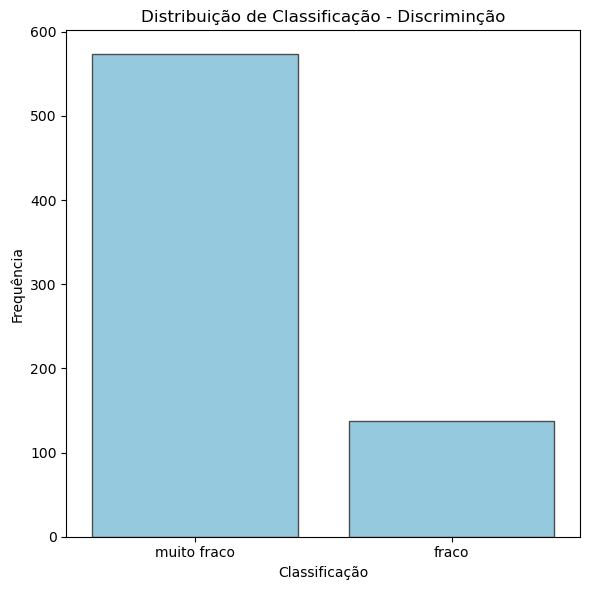
\includegraphics[width=0.62\linewidth]{Figures/Classification/2/Classificacao_Discriminacao.png}
    \caption{Distribuição de frequências para a variável discriminação}
    \label{fig:grafico_freq_discriminacao}
\end{figure}



\begin{table}[!h]
    \centering
\begin{small}    
    \caption{Reclassificação de questões segundo o poder de discriminação para a base de questões utilizada}
    \label{tab:discriminacao_prog}
    \begin{tabular}{cc}
        \toprule
        \textbf{Valor de $r_{pb}$} & \textbf{Classificação} \\
        \toprule
        $>$ 0,09 & Fraco \\
        $\le$ 0,09 & Muito fraco \\
        \bottomrule
    \end{tabular}
\end{small}
\end{table}


% jackson 
\subsection{Métricas de Avaliação}

Com base nos trabalhos de \cite{marcos2021,jackson2023}, as métricas utilizadas na etapa de classificação foram: acurácia, precisão, revocação, f1-score (macro) e f1-score (micro). Já na etapa de discriminação, foram utilizadas as seguintes métricas: MAE (Mean Absolute Error), RAE (Relative Absolute Error), RSE (Root Squared Error) e $R^2$ (Coeficiente de Determinação).

%===========================================================
\section{Resultados e Discussão}

% Aqui abordaremos a execução final dos códigos de processamento, os dados de dificuldade e discriminação obtidos e o que esses números representam na prática - caracterização e a medição dos parâmetros. Aqui podem entrar alguns gráficos também.

Os resultados obtidos são apresentados e discutidos conforme as questões de pesquisa que nortearam este trabalho.

%=========================================================================

\subsection{Correlação entre variáveis dependentes e independentes}
\label{sec:correlacao_variaveis}

O primeiro estudo realizado atenta a correlação entre as variáveis independentes e dependentes. Como este estudo já foi realizado anteriormente por \cite{marcos2021,elrik2022,jackson2023}, o grande objetivo desta seção foi aferir se é possível respondermos a QP1, e caso positivo, aferir como a discriminação correlacionaria com os outros indicadores estudados --- especialmente com a taxa de erro, objeto central da QP2. Verificou-se que a discriminação não aparenta ter fortes correlações com nenhum dos outros doze atributos\footnote{A matriz de correlação completa pode ser vista em \url{https://anonymous.4open.science/r/questions-irt-calculator-D6DE/README.md.}}; aparenta ter discriminação moderada com a taxa de erro ($-$0,52) e com a taxa de aceitação ($+$0,44) --- o que pode nos levar a hipótese que itens com maior taxa de erro tendem a discriminar de uma forma pior e vice-versa (o que esclarece a QP3); além de apresentar uma correlação moderada para o tempo de implementação ($-$0,38), mostrando que questões que demandam um tempo maior de implementação tendem a ser menos discriminatórias. Além disso, destacam-se o número de submissões e o número de testes com um índice de correlação baixo, demonstrando que estes atributos não interferem no poder discriminatório.

% \begin{figure}
%     \centering
%     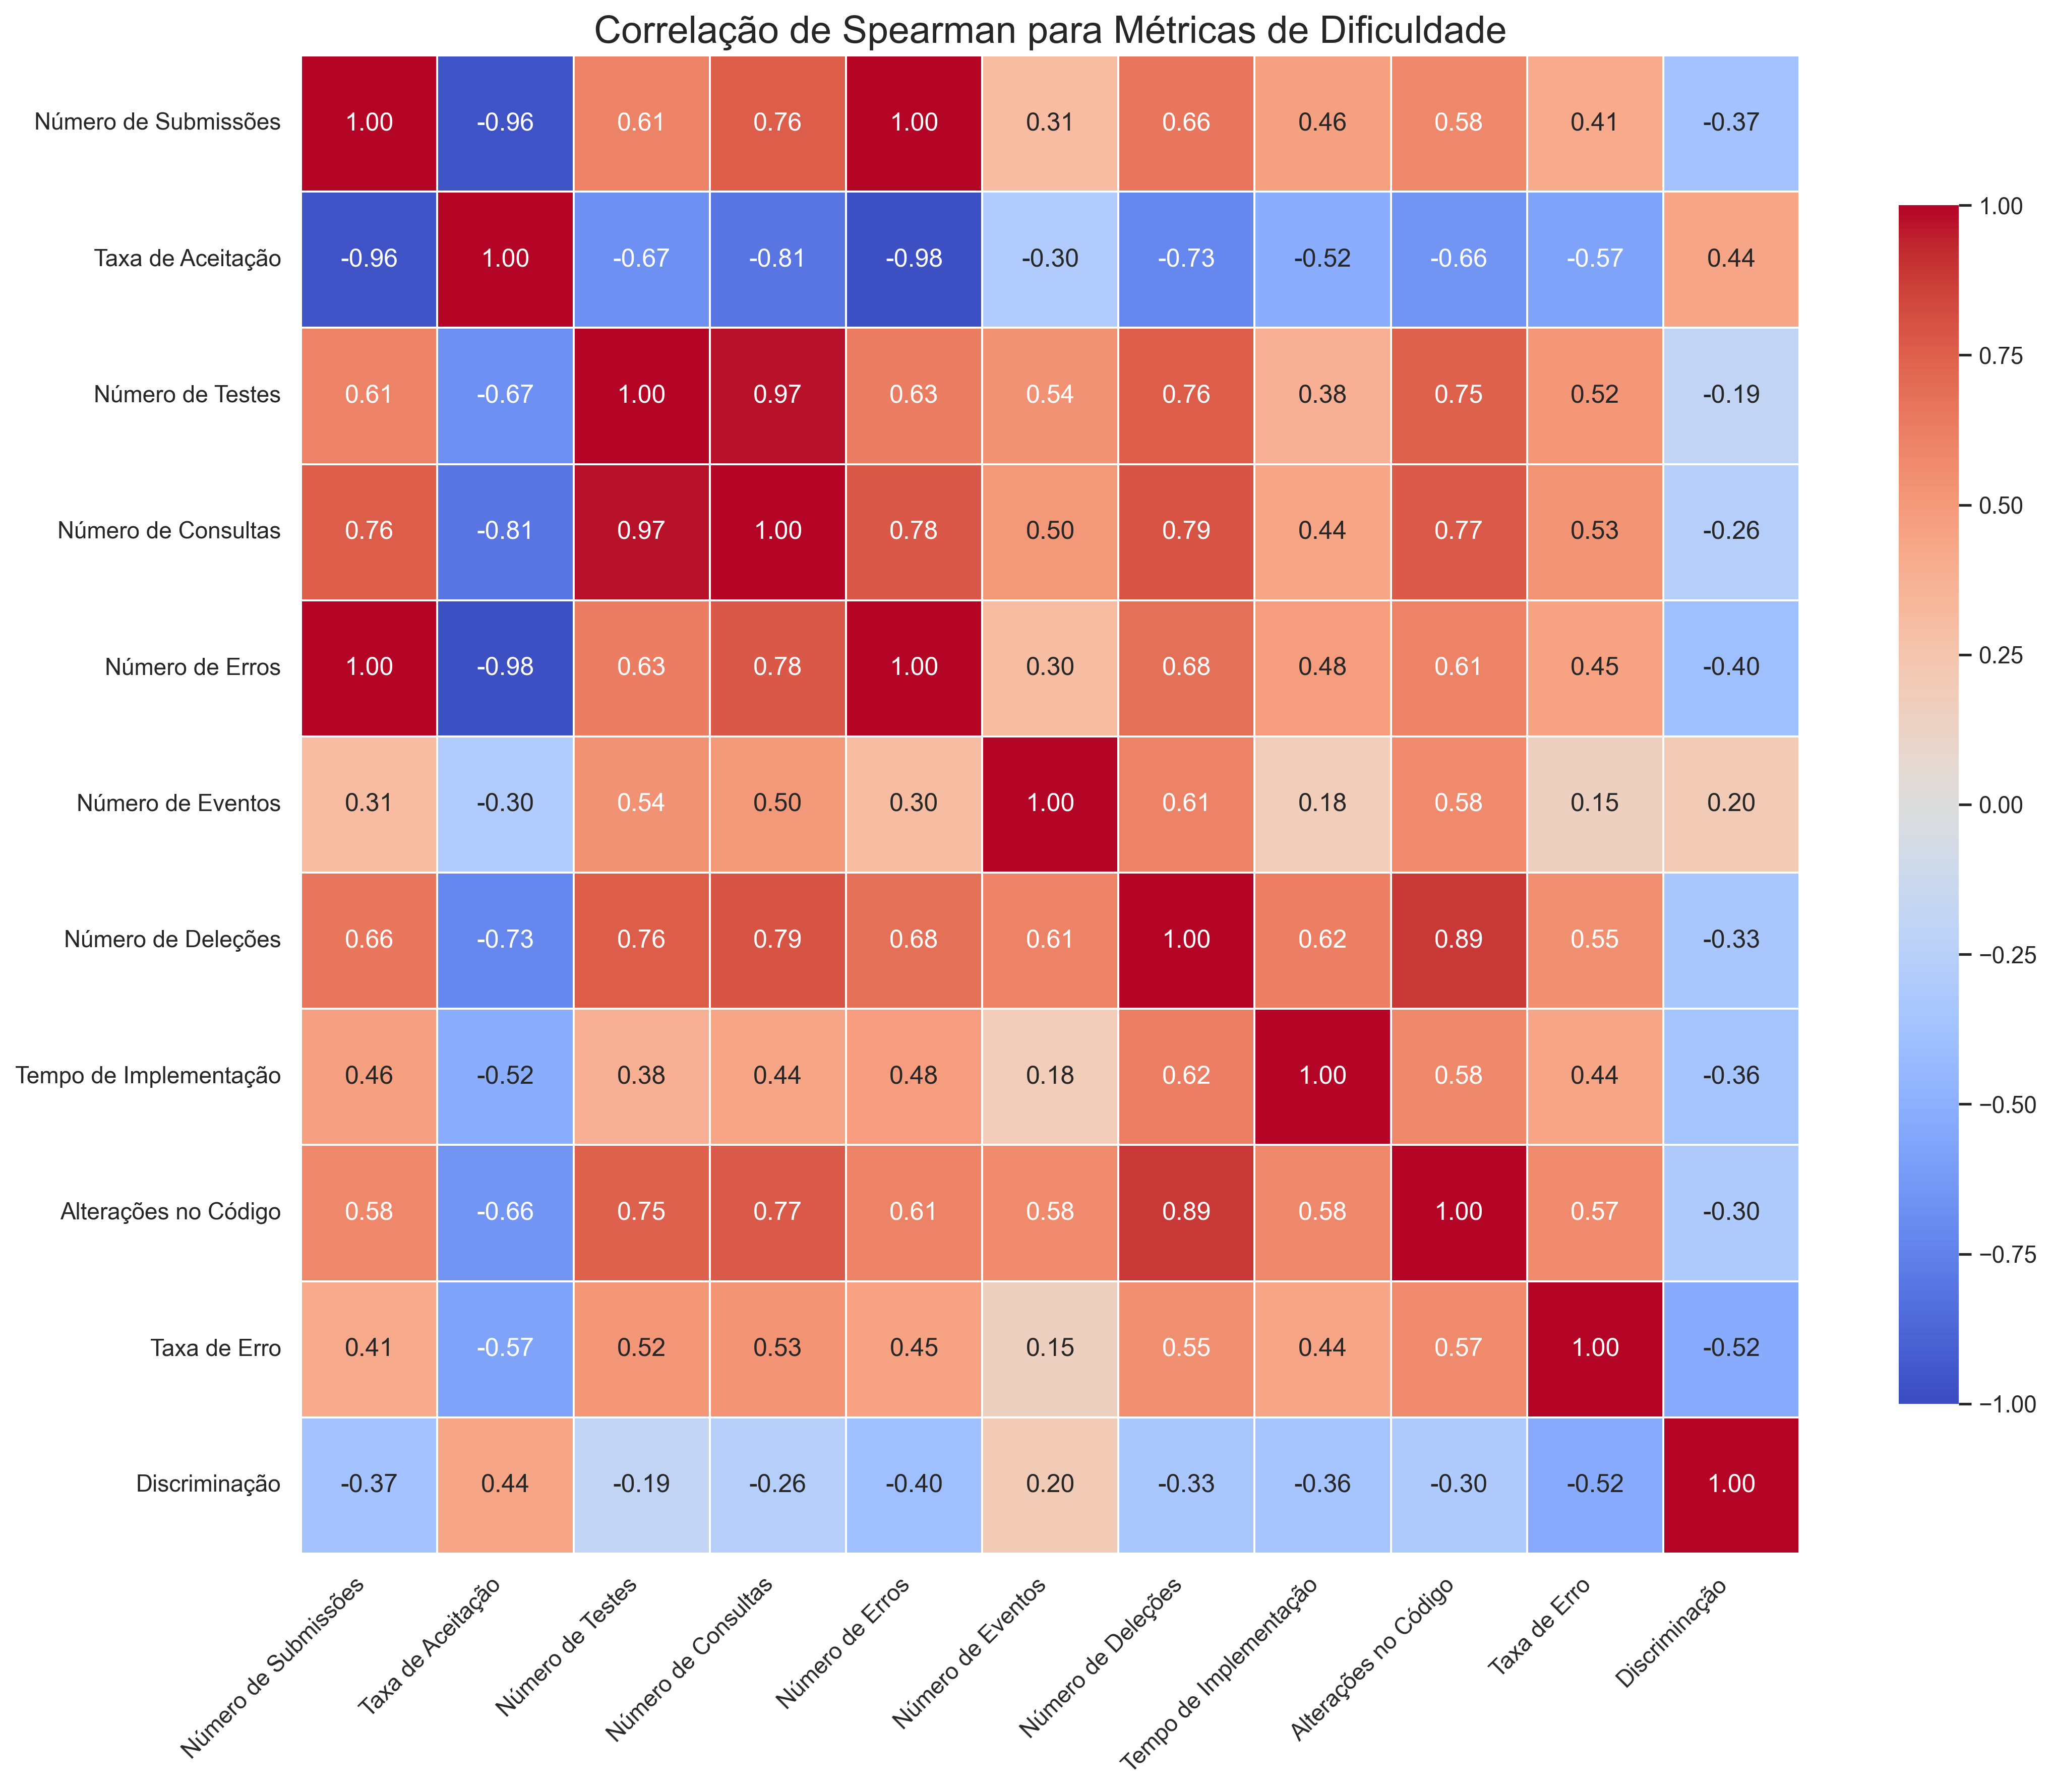
\includegraphics[width=1.0\linewidth]{Figures/Correlations/Correlação_de_Spearman_para_Métricas_de_Dificuldade.png}
%     \caption{Correlação de Spearman para as métricas de dificuldade}
%     \label{fig:correlacao_discriminacao}
% \end{figure}


\subsection{Precisão das métricas de dificuldade}

O segundo estudo faz ligação aos modelos de classificação e regressão estudados. Primeiramente, são apresentados os resultados obtidos para os modelos de regressão utilizados na previsão das métricas de dificuldade. Vale destacar que para cada métrica de dificuldade, listamos o modelo que gerou o melhor resultado. A Tabela~\ref{tab:tabela_regressao} sumariza os desempenhos dos modelos em termos de diversas métricas estatísticas, incluindo $R^2$ ajustado, MAE, RAE, RSE e o $R^2$. Notamos que, para a discriminação, o modelo Extreme Gradient Boosting alcançou o melhor $R^2$ ajustado, com um valor de 0,61, destacando-se como a melhor opção para esta tarefa.

\begin{table}[h!]
    \centering
    \caption{Resultados para o modelo de regressão}
    \resizebox{\textwidth}{!}{%
    \begin{tabular}{llccccc}
        \toprule
        \textbf{Métrica de dificuldade} & \textbf{Modelo} & \textbf{R² ajustado} & \textbf{MAE} & \textbf{RAE} & \textbf{RSE} & \textbf{R²} \\
        \midrule
        Número de submissões     & Random Forest               & 0,18 & 1,47   & 0,80 & 0,81 & 0,19 \\
        Taxa de aceitação     & Extreme Gradient Boosting   & 0,42 & 0,09   & 0,75 & 0,57 & 0,43 \\
        Número de testes         & Random Forest               & 0,42 & 3,53   & 0,72 & 0,57 & 0,43 \\
        Número de consultas      & Random Forest               & 0,41 & 4,50   & 0,73 & 0,58 & 0,42 \\
        Número de erros           & Random Forest               & 0,20 & 1,49   & 0,78 & 0,79 & 0,21 \\
        Número de eventos        & Random Forest               & 0,31 & 349,88 & 0,74 & 0,68 & 0,32 \\
        Número de eventos de deleção    & Random Forest               & 0,53 & 24,44  & 0,66 & 0,46 & 0,54 \\
        Tempo de implementação & Random Forest              & 0,52 & 133,10 & 0,59 & 0,47 & 0,53 \\
        Quantidade de alterações no código  & Random Forest           & 0,69 & 145,55 & 0,56 & 0,30 & 0,70 \\
        Taxa de erro     & Random Forest               & 0,48 & 9,60   & 0,66 & 0,51 & 0,49 \\
        Discriminação       & Extreme Gradient Boosting   & 0,61 & 0,02   & 0,56 & 0,38 & 0,62 \\
        \bottomrule
    \end{tabular}%
    }
    \label{tab:tabela_regressao}
\end{table}

As Tabelas~\ref{tab:tabela_class_binaria} e~\ref{tab:tabela_class_ternaria} mostram o desempenho obtido pelos modelos ao categorizar as predições em dois e três níveis de dificuldade, respectivamente. Buscando melhor esclarecimento para a QP2, realizamos experimentos para as duas categorizações. Após a realização dos testes, observou-se que taxa de erro obteve resultados melhores na classificação binária, com um f1-micro de 0,81. Porém, a discriminação teve um desempenho levemente superior na classificação ternária, com 0,90 de f1-micro contra 0,89 da classificação binária. Tal qual no trabalho de \cite{jackson2023}, a queda de desempenho ao se fazer a classificação ternária em comparação à classificação binária é evidente, apesar da nova métrica, a discriminação, ter mantido um limiar estável.

\begin{table}[h!]
    \centering
    \small
    \caption{Resultados da classificação binária (duas classes de dificuldade)}
    \label{tab:tabela_class_binaria}
    \begin{tabular}{lccl}
        \toprule
        \textbf{Métrica de dificuldade} & \textbf{f1-micro} & \textbf{Acurácia} & \textbf{Classificador} \\
        \midrule
        Discriminação       & 0,89 & 0,83 & Random Forest \\
        Taxa de erro       & 0,81 & 0,74 & Extreme Gradient Boosting \\
        Tempo de implementação & 0,78  & 0,78 & Extreme Gradient Boosting \\
        Quantidade de alterações no código & 0,77 & 0,77   & Gradient Boosting \\
        Número de eventos         & 0,73  & 0,73 & Random Forest \\
        Taxa de aceitação      & 0,72 & 0,71 & Extreme Gradient Boosting \\
        Número de eventos de deleção    & 0,71  & 0,71 & Extreme Gradient Boosting \\
        Número de erros           & 0,70 & 0,70 & Extreme Gradient Boosting \\
        Número de consultas       & 0,70 & 0,70 & Extreme Gradient Boosting \\
        Número de submissões      & 0,68 & 0,68 & Gradient Boosting \\
        Número de testes          & 0,68 & 0,68 & Gradient Boosting \\
        \bottomrule
    \end{tabular}
\end{table}

\begin{table}[h!]
    \centering
    \small
    \caption{Resultados da classificação ternária (três classes de dificuldade)}
    \label{tab:tabela_class_ternaria}
    \begin{tabular}{lccl}
        \toprule
        \textbf{Métrica de dificuldade} & \textbf{f1-micro} & \textbf{Acurácia} & \textbf{Classificador} \\
        \midrule
        Discriminação        & 0,90 & 0,84 & Extreme Gradient Boosting \\
        Tempo de implementação & 0,67 & 0,67 & Random Forest \\
        Quantidade de alterações no código & 0,63 & 0,63 & Extreme Gradient Boosting \\
        Taxa de erro       & 0,63 & 0,62 & Gradient Boosting \\
        Número de eventos         & 0.61 & 0.60 & Extreme Gradient Boosting \\
        Taxa de aceitação      & 0,59 & 0,58 & Gradient Boosting \\
        Número de eventos de deleção    & 0,56 & 0,56 & Gradient Boosting \\
        Número de testes          & 0,54 & 0,54 & Random Forest \\
        Número de consultas       & 0,52 & 0,52 & Random Forest \\
        Número de submissões      & 0,52 & 0,51 & Extreme Gradient Boosting \\
        Número de erros           & 0,50 & 0,50 & Extreme Gradient Boosting \\
        \bottomrule
    \end{tabular}
\end{table}

\subsection{Limitações}

Como demonstrado na Seção~\ref{sec:calculo_disc}, uma limitação enfrentada foi a discriminação baixa na maioria das questões da base usada (Fraco ou Muito Fraco). Tal fato pode ter sido ocasionado pela base de questões conter apenas disciplinas de programação introdutória, onde o objetivo é familiarizar o discente com as linguagens de programação através de exemplos simples e preceitos básicos, como laços, condicionais e leitura de entradas do usuário. Assim, é plausível assumir a hipótese de que questões introdutórias de programação não são um bom limiar para realizar a classificação de um espaço amostral de alunos, visto que estas não possuem um alto poder discriminatório. %Isto pode implicar que, em uma aplicação real deste sistema, os resultados serem considerados insatisfatórios pelos docentes responsáveis por tais disciplinas.

Além disso, como observado por \cite{elrik2022,jackson2023}, outra limitação é que a base de questões provém de um único JO, prejudicando a replicabilidade das observações. %, visto que os ambientes de aprendizagem são distintos entre si (outra metodologia de ensino, outro método de avaliação, outra carga horária de aulas, etc.).
Ademais, outra limitação encontrada foi o número reduzido de questões disponíveis. Como elas são empregadas apenas em atividades avaliativas e são distribuídas aleatoriamente entre os discentes para evitar plágio, algumas são distribuídas com mais frequência do que outras, causando um desequilíbrio na base de dados.
%Como destacado por \cite{marcos2021}, questões com menos de dezesseis respostas são consideradas não ideais para a análise dos indicadores apresentados. 

%===========================================================
\section{Conclusão e Trabalhos Futuros}

Este trabalho teve como objetivo adaptar a TRI aos algoritmos preditores de classificação de questões, adicionando uma nova variável dependente, a discriminação, e a adaptação de uma variável existente, a taxa de erro. Após a definição dos objetivos, foram utilizados algoritmos de aprendizagem de máquina para calcular as variáveis dependentes e independentes --- sendo estas analisadas e classificadas por meio do uso de dois grupos de algoritmos: os de classificação e os de regressão.

Um ponto bem-sucedido neste trabalho foi a robustez na predição da discriminação, tanto em duas, como em três categorias, apesar da base desbalanceada de dados e da fraca discriminação na amostra de questões analisadas. Como visto anteriormente no trabalho de \cite{jackson2023}, mesmo com o aumento da base de dados em relação a trabalhos anteriores, não é possível elucidar a dificuldade de uma questão a partir de um único atributo de código, mesmo atualizando a taxa de erro e adicionando a discriminação. Isto leva aos experimentos usando algoritmos de classificação e regressão.

Embora a correlação entre taxa de erro e discriminação tenha sido moderada ($-$0,52), os demais indicadores apresentaram correlações fracas. Isso sugere que a relação entre dificuldade e discriminação pode ser mais complexa do que inicialmente previsto, reforçando a importância de usar bases mais equilibradas e diversificadas para validar essa hipótese. O trabalho não apenas confirma a viabilidade de aplicar a TRI em contextos de avaliação de aprendizagem em programação, mas também abre caminhos para novas investigações, como uso de itens de disciplinas mais avançadas, bancos de questões de cenários mais diversificados, para melhorar ainda mais a avaliação de habilidades.

\subsection{Trabalhos Futuros}

Um trabalho importante a ser realizado é adicionar mais parâmetros da TRI nas variáveis dependentes, e verificar se estas novas variáveis influenciam no cálculo da dificuldade de um item. Como visto anteriormente, a TRI tem quatro parâmetros, sendo os dois não utilizados no trabalho o acerto e o erro ao acaso. Como o acerto ao acaso certamente terá um índice baixo, o erro ao acaso --- que é quando o discente comete uma falha básica na produção de código, pode ser uma boa métrica a ser adicionada.

Uma futura contribuição relevante também seria a possibilidade de estimarmos a habilidade de um item ou de um aluno em específico. De acordo com \cite{Liz2020}, a estimativa da habilidade está relacionada com a probabilidade de o sujeito responder corretamente aos itens, considerando um ou mais parâmetros. Para calcularmos a habilidade, podem ser usados diferentes modelos matemáticos, dependendo do 
número de parâmetros envolvidos, da dimensionalidade ou do tipo de itens presente no instrumento. Com estes novos itens, será possível recalcular a discriminação já existente de forma mais precisa, adicionando novos itens à fórmula. 

Outra abordagem futura é o aumento e diversificação da base de questões. Como mostrado nas seções anteriores, a mostra usada neste trabalho utilizou questões de programação introdutória, de baixo poder discriminatório ($<$ xxx). Caso seja possível utilizar questões de disciplinas mais avançadas, como, por exemplo, Estruturas de Dados, o poder discriminatório das questões pode ser mais variado e o balanceamento de categorias das demais métricas pode ser mais equilibrado.

%============================================
%\section*{Agradecimentos}
% Esta pesquisa, realizada no âmbito do Projeto Samsung-UFAM de Ensino e Pesquisa (SUPER), de acordo com o Artigo 39 do Decreto n°10.521/2020, foi financiada pela Samsung Eletrônica da Amazônia Ltda, nos termos da Lei Federal n°8.387/1991, através do convênio 001/2020 firmado com a UFAM e FAEPI, Brasil.


\bibliographystyle{sbc}
\bibliography{sbc-template}

\end{document}